\chapter{Contribution to the solution of elastic-plastic problems in two space dimensions}
%% Faire un historique des formulations faites.
%% Formuler le problème à notre sauce et identifier les cas évoqués en intro en particularisant les modules tangents etc. a ce moment, parler des trajets de chargement et des types d'ondes

\section*{Introduction}
It has been shown throughout this manuscript that hyperbolic problems of solid mechanics are solved in a different manner depending on the numerical explicit method employed. 
In particular, irreversible deformations which are usually computed numerically based on well-known constitutive integrators, may greatly differ from one scheme to another, even for one-dimensional problems.
However, the accurate assessment of residual stresses and strains are of major importance for many industrial applications such as, among others, high-speed metal forming, crash-proof design or the study of earthquakes impact on structures.
The simulations performed in chapter \ref{chap:chap4} emphasized the improvements enabled by the knowledge of the characteristic structure of the solution of conservation laws systems, especially for elastoplastic solids.
Nevertheless, the introduction of the exact solution by means of approximate Riemann solvers is so far only carried out for one-dimensional and specific multi-dimensional loading cases for elastic-plastic solids.

The purpose of this chapter is to provide solutions and cues for future works for more general two-dimensional elastoplasticity problems under small strains. 
More information on the structure of solutions to these problems allow a better understanding of physical phenomena occuring in media on the one hand, and the ability of accurately deal with them numerically on the other hand.
The chapter is organized as follows.
A brief historical review of the solution of plastic waves in two-dimension space is made in section \ref{sec:review}.
Then, the equations of plastic flow, which characteristic analysis is carried out, are recalled in section \ref{sec:charac_plast}.
Attention is next paid in section \ref{sec:stress_paths} to the evolution of stress components through simple waves possibly arising in the solution. 
Some thus identified loading paths are finally discussed in section \ref{sec:ep_Riemman_solver} in the context of the development of dedicated approximate Riemann solvers. 

\section{Historical review}
\label{sec:review}
Until the 50s, researches on dynamic problems in elastic-plastic solids were focused on uni-axial stress or strain, pure bending or pure torsion loading conditions \cite{Taylor,vonKarman}, and were carried out for materials characterization purposes.
The first references that brought some understanding about the response of linearly hardening solids to combined shear and pressure loads are those of Rakhmatulin \cite{Rakhmatulin} and Cristescu \cite{CRISTESCU19591605}.
These early analytical investigations on plane stress impacts in the plastic regime led to the conclusion that elastic waves, as well as plastic combined-stress simple waves, can propagate in two-dimensional solids. 
While the former were well-known, the latter were shown to fall into the two \textit{fast waves} and \textit{slow waves} families.
% It has been moreover shown that the fast waves propagate faster than the plastic pressure discontinuity in uni-axial problems would, for a given compression load amplitude.
% Likewise, slow waves propa
% The maximal value of fast waves (\textit{resp. slow waves}) is higher than that of pressure (\textit{resp. shear}) plastic discontinuity occuring in one-dimensional problems, for a given compression (\textit{resp. shear}) load amplitude.

Later, Bleich and Nelson \cite{Bleich} considered superimposed plane and shear waves in an ideally elastic-plastic materials submitted to step loads.
It has then been highlighted that different loading cases yield different characteristic structures of the solution of a Picard problem, thus revealing the complexity of plastic flows in more than one dimension.
% Distinguer un peu plus ces deux contributions.
%\thomas{see \cite[p.56 pdf]{Nowacki},\cite{Goel}}. 
The same conclusions have been drawn by Clifton \cite{Clifton} for hardening materials under tension-torsion, who furthermore studied the influence of plastic pre-loading on the solution.
This contribution established the existence of loading paths through the simple waves arising from the characteristic analysis of the hyperbolic system.
Indeed, the combined-stress wave nature lies in ODEs which govern the evolution of stress components within the simple waves.
The integration of these equations of the form $d\sigma_{11}=\psi d\sigma_{12}$ allows the building of curves that connect the applied stress state of the Picard problem $(\sigma^d_{11},\sigma^d_{12})$ to the initial state of the medium.
% Indeed, the study mathematical properties of relations between stress components of the form $d\sigma_{11}=\psi d\sigma_{12}$, satisifed inside fast and slow simple waves, allows to connect the applied stress state of the Picard problem $(\sigma^d_{11},\sigma^d_{12})$ to the initial state of the medium.
It has been for instance shown that if a solid is acted upon by a traction force such that $\sigma^d_{11}=0$ and $\sigma^d_{12}$ lies outside the elastic convex, only an elastic shear discontinuity, followed by a slow simple wave, propagates.
Conversely, other loading conditions may lead to the combination of an elastic pressure discontinuity and a fast wave, possibly followed by a slow wave.
Another notable conclusion is that the combined loading paths followed inside simple waves may lead to plastic unloading, whereas only elastic unloading occurs in the one-dimensional theory.
%In addition, it is possible to meet unloading plastic simple waves with contrast to the one-dimensional theory in which the unloading waves propagate at elastic speeds (c'est pas vraiment ça attention).
%Such loading paths are supplemented by ODEs satisfied by the velocity components so that a closed form of the solution of the problem can be derived.

Experimental data collected on a thin-walled tube submitted to a dynamic tensile load \cite{Clifton_exp,Clifton_exp2} confirmed the existence of two distinct families of  simple waves, both involving combined stress paths.
Those works nevertheless exhibited some discrepancies with the theory which have been attributed to the assumption made on the von-Mises yield surface.
As a matter of fact, a constant strain region lying between the fast and slow waves that is predicted by the theory \cite{Clifton} could not be seen in experimental results.
However, by following the endochronic theory of plasticity \cite{Valanis} which does not require the introduction of a yield surface, Wu and Lin \cite{Wu_experimental} obtained numerical results that better fitted the experimental data provided by Lipkin and Clifton \cite{Clifton_exp2}.
The good agreement showed between numerical and experimental results \cite{Wu_experimental} thus confirmed the theory.

Ting and Nan \cite{Ting68} then generalized the work of Bleich and Nelson to hardening materials and Ting \cite{Ting69} widened this of Clifton to more complex loadings, that is a superimposition of one plane wave and two shear waves states.
Once again, the mathematical study of the ODE system governing the stresses evolution inside fast and slow simple waves led to the construction of loading paths in the stress space that depend on the external loads. A review of governing equations for all the cases depending on one space dimension considered above can be found in \cite{Nowacki}.

The information on characteristic structures thus provided has then be used by Lin and Ballman \cite{Lin_et_Ballman} for the development of an iterative Riemann solver.
This procedure is based on successive guesses on the stress state lying in the stationary region so that the loading paths predicted by the theory of Clifton \cite{Clifton} can be integrated numerically until convergence.
The implementation of this solver within a second-order Godunov scheme provided results that were in good agreement with the exact solutions.
Nevertheless, the theoretical investigations mentioned above restrict the development of such numerical tools to problems that depend on one space dimension.
%%
Clifton tackled the solution of plane strain problems in elastic-plastic solids by looking for bi-characteristics \cite{Clifton_thesis} in order to build finite difference schemes that account for plastic waves.
The point of view adopted here is that one can benefit from the simplifications introduced by the writing of Riemann problems in an arbitrary direction of space.
Indeed, the method of characteristics rather than the more complex method of bi-characteristics can be employed with the quasi-linear forms presented in chapter \ref{chap:chap2}.

$\newline$
On the other hand, the existence of plastic shocks in solids under the plane wave assumptions has been investigated by several authors \cite{Mandel1,Germain_shock,Mandel2,Claude}.
In those references high pressure impacts were considered so that the problem may be approximated as falling into the hydrodynamics theory.
Hence, the non-monotonic state law describing the evolution of the hydrostatic pressure is responsible for the creation of shock waves due to colliding characteristics.
%%%%%
This work gave rise to discussions on the internal structure of the shock and more precisely to the nature of the load paths followed in the infinitely thin layer in the vicinity of the shock.
%% Mandel suppose un trajet radial dans le choc et donc s'affranchit de l'analyse de la structure interne.
%% Germain utilise le travail plastic comme variable d'écrouissage. + regarde la structure interne du choc pour compléter les courbes d'hugoniot ?
%% Désaccord sur la variable d'écrouissage
%% Et puis Claude

%% Trajets radiaux + hypothèses sur l'écrouissage

% Structure interne + trajet radial de Mandel



%%% Local Variables:
%%% mode: latex
%%% TeX-master: "../mainManuscript"
%%% End:


\section{Elastic-plastic wave structure in two space dimensions}
\label{sec:charac_plast}
%% Comment the possibility of widening the approach to kinematic hardening ?
\subsection{Governing equations}
We are concerned with linear isotropic hardening materials which elastic domain is given by the von-Mises yield surface, under isothermal deformations in the linearized geometrical framework.
The balance equation of linear momentum with neglected body forces, and the geometrical balance equations are:  
\begin{equation}
  \label{eq:ch5_balance_equations}
  \left\lbrace \begin{aligned}
    %\label{eq:ch5_linear_momentum}
    & \rho \dot{\vect{v}} - \nablav \cdot \tens{\sigma} = \vect{0} \\
    %\label{eq:ch5_linear_momentum}
    &  \dot{\tens{\eps}} - \nablav \cdot \(\frac{\vect{v}\otimes \tens{I} + \tens{I} \otimes \vect{v}}{2}\) = \vect{0} 
  \end{aligned} \right.
\end{equation}
In addition, the elastic-plastic constitutive equations derived from thermodynamics in section \ref{sec:constitutive-equations} are recalled here:
\begin{subequations}
  \label{eq:ch5_plasticity_equations}
  \begin{empheq}[left=\empheqlbrace]{align}
    \label{eq:ch5_von-Mises_yield}
    & f\(\tens{\sigma},\Acb \)= \sqrt{\frac{3}{2}}\norm{\tens{s}} - \(R(p)+\sigma^y\) \equiv 0,\quad \text{with }\tens{s}=\tens{\sigma}-\frac{1}{3}\tr \tens{\sigma} \tens{I} \\
    % \label{eq:ch5_kin_hard}
    % & \tens{Y}=\frac{2}{3}C\tens{\eps}^p \\
    \label{eq:ch5_iso_hard}
    & R(p)=C \: p \\
    \label{eq:elastoplastic_tangent}
    & \tens{\dot{\sigma}}=\(\Cbb^{elast} - \beta\:\tens{s}\otimes\tens{s} \):\tens{\dot{\eps}} = \Cbb^{ep}:\tens{\dot{\eps}} \\
    \label{eq:ch5_plastic_flow}
    & \beta = \frac{6\mu^2}{3\mu +C}\times\frac{1}{\tens{s}:\tens{s}}\\
    \label{eq:ch5_EP_acoustic}
    & A_{ij}^{ep}=  A_{ij}^{elast} -  \beta (n_k s_{ki})(s_{jl}n_l)
  \end{empheq}
\end{subequations}
In the expression of von-Mises yield function \eqref{eq:ch5_von-Mises_yield}, the (positive) linear isotropic hardening law \eqref{eq:ch5_iso_hard} is considered.
Moreover, the elastoplastic acoustic tensor \eqref{eq:ch5_EP_acoustic} is decomposed as an elastic part $A_{ij}^{elast}$ and a plastic part depending on the direction of the plastic flow through the coefficient $\beta$ \eqref{eq:ch5_plastic_flow}.
%At last, the (isotropic)elasticity tensor $\Cbb$ in equation \eqref{eq:elastoplastic_tangent} can be inverted to yield the following elastic law:
By inverting the (isotropic)elasticity tensor $\Cbb$ involved in equation \eqref{eq:elastoplastic_tangent}, the following elastic law is written in the isotropic case:
\begin{equation}
  \label{eq:ch5_elastic_inverse}
  \tens{\eps}^e = \frac{1+\nu}{E} \tens{\sigma} - \frac{\nu}{E} \tr \tens{\sigma} \tens{I}
\end{equation}
with Young's modulus $E$ and Poisson's ration $\nu$.

The quasi-linear form of the sets of equations \eqref{eq:ch5_balance_equations} and \eqref{eq:ch5_plasticity_equations} in a Cartesian coordinates system and an arbitrary direction $\vect{n}$ is:
\begin{equation}
  \label{eq:ch5_quasilinear_normal}
  \Qcb_t + \Jbsf \drond{\Qcb}{x_n} = \vect{0} 
\end{equation}
where $x_n=\vect{x}\cdot\vect{n}$, $\Qcb=\matrice{\vect{v}\\ \tens{\sigma}}$, and $\Jbsf$ is the Jacobian matrix.
It has been shown in section \ref{sec:characteristic_analysis} that the $3$ eigenvalues $\omega^p$ and eigenvectors $\vect{l}^p$ of the acoustic tensor lead to $6$ left characteristic fields of the Jacobian matrix $\{c_K;\Lcb^K\}$ according to:
\begin{equation}
  \label{eq:ch5_left_eigenfields}
  \left\lbrace \pm \sqrt{\frac{\omega_p}{\rho}} ; \quad \[\: \pm \rho\sqrt{\frac{\omega_p}{\rho}} \vect{l}^p , -\vect{l}^p\otimes \vect{n} \:\]  \right\rbrace ,\quad p=1,2,3
\end{equation}
In addition, three independent left eigenvectors associated to the zero eigenvalue of system \eqref{eq:ch5_quasilinear_normal}, which is of multiplicity $3$, are found by solving:
\begin{equation}
  \label{eq:ch5_null_eigen}
  \tens{\sigma}^K:\(\Cbb^{ep}\cdot  \vect{n}\) =\vect{0},\quad K=1,2,3
\end{equation}

The present formulation differs from those of \textsc{Bleich} \cite{Bleich}, \textsc{Clifton} \cite{Clifton}, and hence these of \textsc{Ting} and \textsc{Nan} \cite{Ting68} and \textsc{Ting} \cite{Ting69}, in that equation  \eqref{eq:ch5_quasilinear_normal} is based on the elastoplastic stiffnesses rather than softenesses.
As a consequence, it will be seen in what follows that the equations can be easily specialized to plane strain and plane stress cases.
%In what follows, the above equations are specified to plane strain and plane stress cases.
\subsection{Problems in two space dimensions}
We now focus on the solid domain $x_1 \times x_2 \times x_3 \in [0,\infty[ \times [-h,h] \times [-e,e]$ in a Cartesian coordinates system, where $e$ and $h$ are arbitrary lengths.
%The solid is subject in the plane $x_1=0$ to a traction force $\vect{T}^1$ restricted to the $(\vect{e}_1,\vect{e}_2)$ plane, that is $T_3=0$.
It is assumed that all quantities depend solely on $x_1$ and $x_2$ except the velocity component $v_3$ that may depend on $x_3$.
In particular, it is the case for $e \ll h$.

The solid is under plane strain conditions, that is $\tens{\eps}\cdot\vect{e}_3=\vect{0}$, if the velocity $\vect{v}$ does not depend on $x_3$ and if $v_3$ vanishes.
Thus, combining the additive partition of the infinitesimal strain tensor: $\tens{\eps}=\tens{\eps}^e+\tens{\eps}^p$, with the elastic law \eqref{eq:ch5_elastic_inverse} and the kinematic condition $\eps_{33}=0$, one gets:
\begin{equation}
  \label{eq:plane_strain_stress33}
  \sigma_{33}=\nu\(\sigma_{11}+\sigma_{22}\) - E\eps^p_{33}
\end{equation}
Hence, the quasi-linear form \eqref{eq:ch5_quasilinear_normal} reduces for plane strain problems to a system of dimension $5$ with unknowns $v_1,v_2, \sigma_{11},\sigma_{12}$, and $\sigma_{22}$.


Alternatively, a plane stress state ($\tens{\sigma}\cdot\vect{e}_3=\vect{0}$) is assumed if the planes $x_3=\pm h$ are traction free and $e\ll h$.
As a result, the stress component $\sigma_{33}$ can be removed from the system \eqref{eq:ch5_quasilinear_normal}.
Nevertheless, the tangent modulus must account for the vanishing out-of-plane stress component.
Specialization of equation \eqref{eq:elastoplastic_tangent} to $\sigma_{33}$ yields:
\begin{equation*}
  \dot{\sigma}_{33}=C^{ep}_{33ij} \dot{\eps}_{ij} =0
\end{equation*}
from which one writes:
\begin{equation*}
  C^{ep}_{3333} \dot{\eps}_{33} = - C^{ep}_{33ij}\dot{\eps}_{ij} \quad i,j=\{1,2\}
\end{equation*}
Hence, the constitutive equations are rewritten by means of a two-dimensional tangent modulus $\widetilde{\Cbb}^{ep}$:
\begin{equation}
  \label{eq:CP_constitutive}
  \dot{\sigma}_{ij}=C^{ep}_{ijkl} \dot{\eps}_{kl} - \frac{C^{ep}_{ij33}C^{ep}_{33kl}}{C^{ep}_{3333}}\dot{\eps}_{kl}= \widetilde{C}^{ep}_{ijkl} \dot{\eps}_{kl}\qquad i,j,k,l=\{1,2\} 
\end{equation}
The characteristic structure of the problem is then given by this of the associated acoustic tensor $\tens{\widetilde{A}}^{ep}=\vect{n}\cdot\widetilde{\Cbb}^{ep}\cdot \vect{n}$.

The removal of $\sigma_{33}$ from system \eqref{eq:ch5_quasilinear_normal} for both plane strains and plane stresses allows to solve the problem in a two-dimensional setting.
Then, generically denoting the acoustic tensor by $\tens{A}$, the characteristic structures are given by the eigenvalues:
\begin{subequations}
  \begin{alignat}{1}
    \label{eq:ch5_eigenAcc1}
    &\omega_1 = \frac{1}{2}\(A_{11}+A_{22} + \sqrt{(A_{11}-A_{22})^2+{4A_{12}}^2}\) \\
    \label{eq:ch5_eigenAcc2}
    &\omega_2 = \frac{1}{2}\(A_{11}+A_{22} - \sqrt{(A_{11}-A_{22})^2+{4A_{12}}^2}\)     
  \end{alignat}
\end{subequations}
and the associated eigenvectors:
\begin{equation}
  \label{eq:ch5_eigenvectAcc}
   \vect{l}^1=[ A_{22}-  \omega_1 \:,\: -A_{12}] \qquad ;\qquad  \vect{l}^2=[ -A_{12} \:,\:A_{11}- \omega_2 ]
\end{equation}
From equation \eqref{eq:ch5_left_eigenfields}, we see that two families of waves with celerities $c_f=\pm \sqrt{\omega_1/\rho}$ and $c_s = \pm \sqrt{\omega_2/\rho}$ may travel in the domain.
Those waves are respectively referred to as fast and slow waves.
Note that subtracting equations \eqref{eq:ch5_eigenAcc1} and \eqref{eq:ch5_eigenAcc2} leads to:
\begin{equation}
  \label{eq:diff_celerities}
  \rho c_f^2 - \rho c_s^2 = \sqrt{(A_{11}-A_{22})^2+{4A_{12}}^2} \geq 0
\end{equation}
Hence, the characteristic speed associated to fast waves is always greater than of equal to that of slow waves.

The four left eigenfields of the Jacobian matrix thus read:
\begin{subequations}
  \begin{alignat}{1}
    \label{eq:ch5_Jac_eigenfield_fast}
    &\left\lbrace \pm c_f ; \quad \Lcb^{c_f^\pm}=\[\: \pm \rho c_f \vect{l}^1 , -\vect{l}^1\otimes \vect{n} \:\]  \right\rbrace \\
  \label{eq:ch5_Jac_eigenfield_slow}
    &\left\lbrace \pm c_s ; \quad \Lcb^{c_s^\pm}=\[\: \pm \rho c_s \vect{l}^2 , -\vect{l}^2\otimes \vect{n} \:\]  \right\rbrace
  \end{alignat}
\end{subequations}
where $\Lcb^{c_f^+}$ and $\Lcb^{c_f^-}$ are associated to the right-going and left-going fast waves respectively.
The same goes for $\Lcb^{c_s^+}$ and $\Lcb^{c_s^-}$.
Furthermore, one stationary wave associated to the zero eigenvalue of the Jacobian matrix, and which left eigenvector satisfies equation \eqref{eq:ch5_null_eigen}, has to be added:
\begin{equation}
  \label{eq:ch5_null_left_eigen}
  {\Lcb^0}^T = \matrice{v_1^0 \\[5.pt] v_2^0 \\[5.pt] \sigma_{11}^0 \\[5.pt] \sigma^0_{22} \\[5.pt] \sigma^0_{12} }= \matrice{0 \\[5.pt] 0 \\[5.pt] \(C_{121i}C_{222j}-C_{221i}C_{122j}\)n_in_j \\[5.pt] \(C_{111i}C_{122j}-C_{112i}C_{121j}\)n_in_j \\[5.pt] \(C_{112i}C_{221j}-C_{111i}C_{222j}\)\frac{n_in_j}{2}} = \matrice{0 \\ 0 \\ \alpha_{11} \\ \alpha_{22} \\ \alpha_{12} }
\end{equation}
with $\Cbb=\Cbb^{ep}$ for plain strain and $\Cbb=\widetilde{\Cbb}^{ep}$ for plane stress.
%In particular, $\Cbb$ reduces to the elastic stiffness tensor when no plastic flow occurs so that the characteristic structure involves the speeds of elastic pressure waves $c_1$ and shear waves $c_2$. 

It has been seen in section \ref{sec:SVK_solution} that the solution of non-linear problems may contain shock and/or simple waves.
Nevertheless, we restrict here to simple waves by assuming that: (i) the characteristic speeds satisfy $c_1 \geq c_f \geq c_2 \geq c_s $, where $c_1$ and $c_2$ are the speeds of elastic pressure and shear discontinuities respectively; (ii) $c_f$ and $c_s$ monotonically decrease with the hardening of the material; (ii) the computational domain is in an initial natural, plastic strain free state.

The characteristic equations $\Lcb^K \cdot d\Qcb = 0$ are then written:
\begin{subequations}
  %\label{eq:ch5_ODEs}
  \begin{alignat}{3}
    \label{eq:charac_fr}
    & \rho c_f \vect{l}^1 \cdot d\vect{v} - l^1_i n_j d\sigma_{ij} =0 \qquad && \text{along }\: dx/dt = c_f\\
    \label{eq:charac_fl}
    -& \rho c_f \vect{l}^1 \cdot d\vect{v} - l^1_i n_j d\sigma_{ij} =0 \qquad && \text{along }\: dx/dt = - c_f \\
    \label{eq:charac_sr}
    & \rho c_s \vect{l}^2 \cdot d\vect{v} - l^2_i n_j d\sigma_{ij} =0 \qquad  && \text{along }\: dx/dt =  c_s \\
    \label{eq:charac_sl}
    -& \rho c_s \vect{l}^2 \cdot d\vect{v} - l^2_i n_j d\sigma_{ij} =0 \qquad  && \text{along }\: dx/dt = - c_s \\
    \label{eq:charac_contact}
    &\alpha_{11}d\sigma_{11} + \alpha_{12}d\sigma_{12} + \alpha_{22}d\sigma_{22}=0 \qquad && \text{along }\: dx/dt =0 
  \end{alignat}
\end{subequations}
Integration of equations \eqref{eq:charac_fr} to \eqref{eq:charac_contact} leads to integral curves through simple waves in which several stress components vary, hence the name of combined-stress simple waves \cite{CRISTESCU19591605}.
Following \cite{Clifton}, the method of characteristic is applied by combining equations \eqref{eq:charac_fr} to \eqref{eq:charac_contact}.
\begin{figure}[h!]
  \centering
  \subcaptionbox{Slow simple wave \label{subfig:slowWave}}{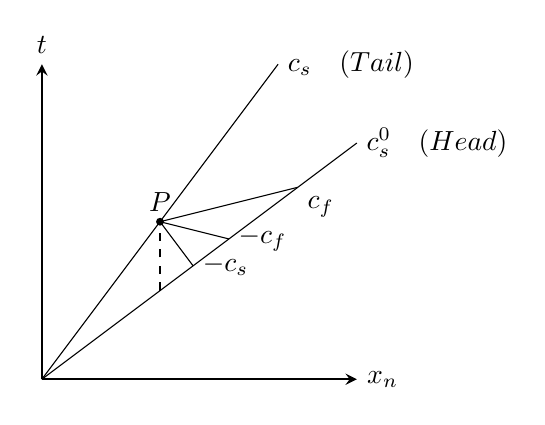
\begin{tikzpicture}[scale=1.,>=stealth] 
  \newcommand\shift{5.}
  %% Slow
  \draw[thick,->] (0,0) -- (4.,0) node[right] {$x_n$};
  \draw[thick,->] (0,0) -- (0.,4) node[above] {$t$};
  % Slope = 0.75
  \draw (0,0) -- (4,3.) node [right] {$c_s^0 \quad (Head)$};
  % Slope = 4./3.
  \draw (0,0) -- (3.,4.) node [right] {$c_s \quad (Tail)$};

  \fill[black] (1.5,1.5*4./3.) circle (0.05) node [above] {$P$};
  %% Other characteristics
  % stationary
  \draw[dashed] (1.5,0.75*1.5) -- (1.5,1.5*4./3.);
  % fast plus (slope =+-0.25)
  \newcommand\px{1.5}
  \newcommand\py{1.5*4./3.}
  \draw (2.*\py-0.5*\px,1.5*\py-3.*\px/8.) node [below right] {$c_f$}-- (1.5,1.5*4./3.) ;
  % fast minus
  \draw (\py+0.25*\px,0.75*\py+3.*\px/16.) node [right] {$-c_f$} -- (1.5,1.5*4./3.) ;
  % slow minus (slope=-4./3.)
  \draw (12.*\py/25.+16.*\px/25.,9.*\py/25.+36.*\px/75.) node [right] {$-c_s$} -- (1.5,1.5*4./3.) ;
\end{tikzpicture}


%%% Local Variables:
%%% mode: latex
%%% TeX-master: "../../mainManuscript"
%%% End:
} \qquad
  \subcaptionbox{Fast simple wave \label{subfig:fastWave}}{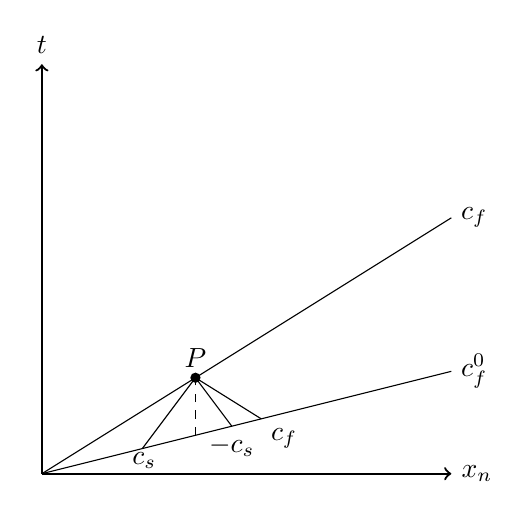
\begin{tikzpicture}[scale=1.3] 
  \newcommand\shift{5.}
  %% Fast
  \draw[thick,->] (0+\shift,0) -- (4.+\shift,0) node[right] {$x_n$};
  \draw[thick,->] (0+\shift,0) -- (0.+\shift,4) node[above] {$t$};
  % Slope = 0.25
  \draw (0+\shift,0) -- (4+\shift,1.) node [right] {$c_f^0$};
  % Slope = 5./8.
  \draw (0+\shift,0) -- (4+\shift,2.5) node [right] {$c_f$};
  
  \fill[black] (1.5+\shift,1.5*5./8.) circle (0.05) node [above] {$P$};
  %% Other characteristics
  \newcommand\pxx{1.5}
  \newcommand\pyy{1.5*5./8.}
  % stationary
  \draw[dashed] (1.5+\shift,1.5/4.) -- (\pxx+\shift,\pyy);
  % fast minus
  \draw (8.*\pyy/7.+5.*\pxx/7.+\shift,2.*\pyy/7.+10.*\pxx/56.) node [below right] {$c_f$}-- (\pxx+\shift,\pyy);
  % slow plus
  \draw (-12.0*\pyy/13.+16.*\pxx/13.+\shift,-3.*\pyy/13.+4.*\pxx/13.) -- (\pxx+\shift,\pyy);
  \node at (-12.0*\pyy/13.+16.*\pxx/13.+\shift+0.02,-3.*\pyy/13.+4.*\pxx/13.-0.12) {$c_s$};
  % slow minus
  \draw (12.0*\pyy/19.+16.*\pxx/19.+\shift,3.*\pyy/19.+4.*\pxx/19.)node [below] {$-c_s$} -- (\pxx+\shift,\pyy);
\end{tikzpicture}


%%% Local Variables:
%%% mode: latex
%%% TeX-master: "../../mainManuscript"
%%% End:
}
  \caption{The method of characteristics through slow and fast simple waves in the $(x_n,t)$ plane.}
  \label{fig:ch5_charac_method}
\end{figure}
The approach consists in tracing every characteristics from some downstream point of a wave where the state vector $\Qcb$ is known, to an upstream point where the solution is seeked. Figures \ref{fig:ch5_charac_method}\subref{subfig:slowWave} and \ref{fig:ch5_charac_method}\subref{subfig:fastWave} schematically illustrate the method for slow and fast simple waves in which the state is known along the head wave and is looked for at point $P$ lying on the tail wave. 
The integral curves through slow and fast simple waves are derived in the next section.

\subsection{Integral curves through simple waves}
The right-going slow waves are first looked at by adding equations \eqref{eq:charac_fr} and \eqref{eq:charac_fl}:
\begin{equation}
  l_i^1 n_j d\sigma_{ij}=0
\end{equation}
Given the geometry of the problem, the vector $\vect{n}$ may be reduced to $\vect{e}_1$ or $\vect{e}_2$.
It therefore comes out:
%In particular, for a vector $\vect{n}$ that is restricted to the axis of the $(\vect{e}_1,\vect{e}_2)$ plane, one gets:
\begin{subequations}
  \begin{alignat}{2}
    \label{eq:sigSlow_n=e1}
    & d\sigma_{11} = - \frac{l^1_2}{l_1^1} d\sigma_{12} = \psi^s_{1}d\sigma_{12} && \qquad \text{for } \:\vect{n}=\vect{e}_1 \\
    \label{eq:sigSlow_n=e2}
    & d\sigma_{22}=- \frac{l_1^1}{l_2^1}  d\sigma_{12} = \psi^s_{2}d\sigma_{12} && \qquad \text{for } \:\vect{n}=\vect{e}_2
  \end{alignat}
\end{subequations}
where $\psi^s_1$ and $\psi^s_2$ are functions of all components of $\tens{\sigma}$. 
Moreover, the $s$ and $f$ superscripts stand for slow and fast waves respectively in the remainder of the manuscript.
With the above equations, the characteristic equation related to the contact wave \eqref{eq:charac_contact} reads:
%Next, the characteristic equation related to the contact wave \eqref{eq:charac_contact} yields:
\begin{subequations}
  \begin{alignat}{2}
    \label{eq:sigContact_n=e1}
    & d\sigma_{22} = -\frac{\psi^s_{1}\alpha_{11}+\alpha_{12}}{\alpha_{22}}d\sigma_{12} && \qquad \text{for } \:\vect{n}=\vect{e}_1 \\
    \label{eq:sigContact_n=e2}
    & d\sigma_{11}= -\frac{\psi^s_{2}\alpha_{22}+\alpha_{12}}{\alpha_{11}} d\sigma_{12} && \qquad \text{for } \:\vect{n}=\vect{e}_2
  \end{alignat}
\end{subequations}
The sets of equations \eqref{eq:sigSlow_n=e1}-\eqref{eq:sigContact_n=e1} and \eqref{eq:sigSlow_n=e2}-\eqref{eq:sigContact_n=e2} show the combined-stress nature of slow simple waves.
% Hence, one stress component may be used as a driving parameter for the two others, as it is the case for $\sigma_{12}$ in equations \eqref{eq:sigSlow_n=e1}, \eqref{eq:sigSlow_n=e2}, \eqref{eq:sigContact_n=e1} and \eqref{eq:sigContact_n=e2}.
On the other hand, the subtraction of equations \eqref{eq:charac_fr} and \eqref{eq:charac_fl} leads to:
\begin{equation*}
  dv_1 = \psi^s_{1}dv_2 = \frac{1}{\psi^s_2}dv_2
\end{equation*}
which, once combined with equations \eqref{eq:sigSlow_n=e1}-\eqref{eq:sigSlow_n=e2} and introduced in \eqref{eq:charac_sl}, yields after simplifications:
\begin{subequations}
  \begin{alignat}{2}
    \label{eq:vSlow_n=e1}
    & dv_1 = -\frac{d\sigma_{11}}{\rho c_s^2} \quad ;\quad  dv_2 = -\frac{d\sigma_{12}}{\rho c_s^2} \qquad & \text{for } \vect{n}=\vect{e}_1\\
    \label{eq:vSlow_n=e2}
    & dv_1 = -\frac{d\sigma_{12}}{\rho c_s^2} \quad ;\quad  dv_2 = -\frac{d\sigma_{22}}{\rho c_s^2} \qquad & \text{for } \vect{n}=\vect{e}_2
  \end{alignat}
\end{subequations}

\begin{remark}
  The integral curves through a left-going slow wave result from the combination of equations \eqref{eq:sigSlow_n=e1}-\eqref{eq:sigSlow_n=e2} introduced in \eqref{eq:charac_sr} rather than \eqref{eq:charac_sl}.
  Therefore, the only difference lies in the signs in equations \eqref{eq:vSlow_n=e1} and \eqref{eq:vSlow_n=e2}
\end{remark}

Similar results are obtained for right-going fast simple waves by using $\vect{l}^2$ instead of $\vect{l}^1$ and $c_f$ rather than $c_s$.
%However, the integral curves involve $\vect{l}^2$ and $c_f$ instead of $\vect{l}^1$ and $c_s$. 
Hence, the evolution in slow and fast waves is governed by the \textit{loading functions}:
\begin{equation}
  \label{eq:loading_func}
  \psi^s_{1}=- \left.\frac{l^1_2}{l_1^1}\right\rvert_{\vect{n}=\vect{e}_1}\quad ,\quad  \psi^s_{2}=- \left.\frac{l_1^1}{l_2^1}\right\rvert_{\vect{n}=\vect{e}_2} \quad ,\quad \psi^f_1=-\left.\frac{l_2^2}{l_1^2}\right\rvert_{\vect{n}=\vect{e}_1} \quad ,\quad \psi^f_2=-\left.\frac{l_1^2}{l_2^2}\right\rvert_{\vect{n}=\vect{e}_2}
\end{equation}
The equations satisfied across right-going slow and fast simple waves are summarized in table \ref{tab:simpleWavesEquations}.
\begin{table}[h!]
  \centering
  \begin{tabular}{cc|ccN}
    \hline
    \multicolumn{2}{c}{Right-going slow wave} \vline& \multicolumn{2}{c}{Right-going fast wave} & \\
    $\vect{n}=\vect{e}_1$ & $\vect{n}=\vect{e}_2$ & $\vect{n}=\vect{e}_1$ & $\vect{n}=\vect{e}_2$&\\
    \hline
    \hline
    $dv_1 = -\frac{d\sigma_{11}}{\rho c_s^2}$ &  $dv_1 = -\frac{d\sigma_{12}}{\rho c_s^2}$ &$dv_1 = -\frac{d\sigma_{11}}{\rho c_f^2}$ &  $dv_1 = -\frac{d\sigma_{12}}{\rho c_f^2}$ &\\ [8pt]
    $dv_2 = -\frac{d\sigma_{12}}{\rho c_s^2}$ & $dv_2 = -\frac{d\sigma_{22}}{\rho c_s^2}$ & $dv_2 = -\frac{d\sigma_{12}}{\rho c_f^2}$ & $dv_2 = -\frac{d\sigma_{22}}{\rho c_f^2}$& \\ [8pt]
    $d\sigma_{11} = \psi^s_{1}d\sigma_{12}$&$d\sigma_{11}= -\frac{\psi^s_{2}\alpha_{22}+\alpha_{12}}{\alpha_{11}} d\sigma_{12}$ &  $d\sigma_{11} = \psi^f_{1}d\sigma_{12}$&$d\sigma_{11}= -\frac{\psi^f_{2}\alpha_{22}+\alpha_{12}}{\alpha_{11}} d\sigma_{12}$ & \\[8pt]
    $d\sigma_{22} = -\frac{\psi^s_{1}\alpha_{11}+\alpha_{12}}{\alpha_{22}}d\sigma_{12}$ & $d\sigma_{22}= \psi^s_{2}d\sigma_{12}$ & $d\sigma_{22} = -\frac{\psi^f_{1}\alpha_{11}+\alpha_{12}}{\alpha_{22}}d\sigma_{12}$ & $d\sigma_{22}= \psi^f_{2}d\sigma_{12}$ & \\[8pt]
    % & & \\
    % & & \\    
    \hline
\end{tabular}
%%% Local Variables:
%%% mode: latex
%%% TeX-master: "../manuscript"
%%% End:

  \caption{Summary of the ODEs satisfied inside right-going slow and fast simple waves.}
  \label{tab:simpleWavesEquations}
\end{table}

The integration of equations gathered in table \ref{tab:simpleWavesEquations} should provide the complete solution of a given problem by means of integral curves or loading paths.
For instance, the velocity resulting from the passage of right-going waves in the direction $\vect{e}_1$ obeys:
\begin{equation}
  \label{eq:integral_example}
  v_1 = v_1^0 - \int_{\tens{\sigma}^0}^{\tens{\sigma}} \frac{d \sigma_{11}}{\rho c^2} \quad ;\quad v_2 = v_2^0 - \int_{\tens{\sigma}^0}^{\tens{\sigma}} \frac{d \sigma_{12}}{\rho c^2}
\end{equation}
where the zero superscript denotes the downstream state.
Nevertheless, \textsc{Clifton} \cite{Clifton} emphasized that depending on the loading conditions, only one simple waves or both may arise in the solution.
Therefore, it is crucial to identify the stress path followed to properly compute integrals \eqref{eq:integral_example}.
%It is thus important to qualify the stress paths through fast and slow waves in order to properly define the upper bound of the integrals of the form \eqref{eq:integral_example}.
This is the purpose of the next section.



%%% Local Variables:
%%% mode: latex
%%% TeX-master: "../mainManuscript"
%%% End:


\section{Loading paths through simple waves}
\label{sec:stress_paths}
% On ne regarde qu'une dimension spatiale en faisant des hypothèse sur les champs alors que nous on se limite à une direction particulière $\vect{n}$.
% En plus, on se limite à l'étude d'ondes simples alors que des chocs peuvent exister (voir Mandell car il semble y etre démontré que les shock n'arrivent que pour $\tau=0$).
% Il y a la question des vitesses charactéristiques plastiques... sont-elles collées aux vitesses élastiques ?
% dependance des vitesses caractéristiques à l'angle entre la direction principale de sigma et la direction de propagation, c'est dit dans la thèse de Clifou en page 90.

\subsection{Properties of the loading paths}
The stress paths followed within slow and fast simple waves are governed by the mathematical properties of the loading functions \eqref{eq:loading_func}.
Before specializing the discussion to plane stress and plane strain cases, some general properties holding regardless of the loading conditions are highlighted.
%The analysis is here carried out for the special case $\vect{n}=\vect{e}_1$, similar results being obtained for the other situation $\vect{n}=\vect{e}_2$.

First, the functions satisfy the orthogonality properties: $\psi^s_1\psi^f_1=-1$ and $\psi^s_2\psi^f_2=-1$.
Indeed, considering the left eigenvectors of the acoustic tensor given in equation \eqref{eq:ch5_eigenvectAcc}, the product $\psi^s_1\psi^f_1$ reads:
\begin{equation*}
  \psi^s_1\psi^f_1 = \frac{l^1_2}{l^1_1}\: \frac{l_2^2}{l^2_1} = \frac{(A_{11}-\omega_2)A_{12}}{(A_{22}-\omega_1)A_{12}}
\end{equation*}
Introduction of the expressions of eigenvalues $\omega_i$ from equations \eqref{eq:ch5_eigenAcc1} and \eqref{eq:ch5_eigenAcc1} further leads to:
\begin{equation*}
  \psi^s_1\psi^f_1 = \frac{A_{11} -A_{22} +\sqrt{(A_{11} -A_{22} )^2 + 4A_{12}^2 }}{A_{22} -A_{11} -\sqrt{(A_{11} -A_{22} )^2 + 4A_{12}^2 }}=-1
\end{equation*}
or equivalently, $\vect{l}^1 \cdot \vect{l}^2=0$.
%as expected by the symmetry of $\tens{A}$.
This orthogonality has already been noticed for particular plane strain and plane stress cases \cite{Clifton,Ting68}. % but now obviously appears as true for all problems in two space dimensions.
However, the eigenvectors of symmetric second-order tensors all satisfy this property in such a way that it is valid for all problems in two space dimensions.
As a result, the study can be restricted to one function in each direction, say $\psi_1^s$ and $\psi_2^s$.

Second, if the function $\psi_1^s$ vanishes at some point of the stress space, the projection of the loading path followed inside a slow wave in the $(\sigma_{11},\sigma_{12})$ plane is vertical according to the ODE \eqref{eq:sigSlow_n=e1}.
Conversely, if $\psi_1^s\rightarrow \infty$, the loading path is horizontal in the $(\sigma_{11},\sigma_{12})$ plane.
%Looking for vanishing $\psi^f_1$ or $1/\psi^f_1$ amounts to finding roots of the components of $\vect{l}^2$:
These situations respectively correspond to:
\begin{subequations}
  \begin{alignat}{1}
    \label{eq:first_root}
    \psi_1^s = 0   & \Leftrightarrow A_{12} =0  \\
    \label{eq:second_root}
    \psi_1^s \rightarrow \infty & \Leftrightarrow A_{22} -\omega_1 =0
  \end{alignat}
\end{subequations}
In particular, if $A_{12}=0$ the second equation reads:
\begin{equation}
  A_{22} -\omega_1 = \frac{1}{2}\(A_{22} -A_{11} -\sqrt{(A_{11} -A_{22} )^2 + 4A_{12}^2 }\) = -\left\langle A _{11}-A _{22}  \right\rangle
\end{equation}
where $\left\langle \bullet \right\rangle$ denotes the positive part operator.
Hence, if $A_{12} =0$ and $A_{11} \neq A_{22} $, one has $\psi^s_1 =0$ and hence $\psi^f_1 \rightarrow -\infty $.
If moreover $A_{11}  = A_{22} $, both components of the eigenvectors vanish and the functions $\psi^s_1$ and $\psi^f_1$ are undetermined.
At last, it follows from equation \eqref{eq:diff_celerities} that the simultaneous satisfaction of conditions \eqref{eq:first_root} and \eqref{eq:second_root} leads to characteristic speeds of simple waves that are identical. Hence, the situation $c_f=c_s$ corresponds to a loss of hyperbolicity of the system.
% Hence, if $A_{12} =0$ and $A_{11} \neq A_{22} $, one has $\psi^s_1 =0$ and $\psi^f_1 \rightarrow \infty $, so that the stress path in the ($\sigma_{11},\sigma_{12}$) plane are vertical (\textit{resp. horizontal}) through a slow (\textit{resp. fast}) wave. 

Analogously, the function $\psi_2^s$ is such that:
\begin{subequations}
  \begin{alignat}{1}
    \label{eq:first_root_psi2cp}
    \psi_2^s \rightarrow \infty  & \Leftrightarrow A_{12} =0  \\
    \label{eq:second_root_psi2cp}
    \psi_2^s =0 & \Leftrightarrow A_{22} -\omega_1 =0
  \end{alignat}
\end{subequations}
Therefore, if both conditions \eqref{eq:first_root_psi2cp} and \eqref{eq:second_root_psi2cp} are satisfied, the system is no longer hyperbolic with characteristic speeds of fast and slow waves that are identical.

According to the ODEs of table \ref{tab:simpleWavesEquations}, the particular values of the loading functions $\psi_i^{s,f}$ through the simple waves propagating in direction $\vect{e}_i$ for $i=\{1,2\}$, provide information about the loading paths in stress space.
First, $\psi_i =0$ leads to $d\sigma_{ii}=0$ (no sum on $i$) so that the longitudinal stress is constant within the simple wave.
Conversely, with loading functions tending to infinity, the stress $\sigma_{12}$ does not vary.
Notice that the coefficients $\alpha_{ij}$ of the left eigenvector of the Jacobian matrix associated to the zero eigenvalue \eqref{eq:ch5_null_left_eigen} also have to be regarded.
Nevertheless, those terms resulting from products of the components of the elastoplastic tangent modulus have complex expressions and are assumed to have non-zero values in the remainder of the manuscript.

The above discussions are now specified to plane strain and plane stress, for which loading conditions leading to $A_{12} =0$ and $A _{11}-A _{22}=0$ are identified.



\subsection{The plane strain case}
The case of plane strain is first considered by using the elastoplastic tangent modulus so that the components of the acoustic tensor for $\vect{n}=\vect{e}_1$ read:
%The elastoplastic tangent modulus under consideration is now that given in equation \eqref{eq:elastoplastic_tangent}, so that the components of the acoustic tensor for $\vect{n}=\vect{e}_1$ read: 
\begin{subequations}
  \begin{alignat}{1}
    \label{eq:DP_A11}
    & A_{11}^{ep}= C_{1111}^{ep} = \lambda + 2\mu -\beta s_{11}^2 \\
    \label{eq:DP_A22}
    & A_{22}^{ep}= C_{2121}^{ep}= \mu -\beta s_{12}^2 \\
    \label{eq:DP_A12}
    & A_{12}^{ep}= C_{1121}^{ep}=-\beta s_{11}s_{12}
  \end{alignat}
\end{subequations}
The associated eigenvalues are then:
\begin{subequations}
  \label{eq:eigen_acc_DP}
  \begin{alignat}{1}
    \label{eq:eigen_acc_DP1}
    & \rho c_s^2 = \frac{1}{2}\( \lambda +3\mu -\beta (s_{11}^2+ s_{12}^2) - \sqrt{(\lambda + \mu -\beta (s_{11}^2-s_{12}^2) )^2 +4(\beta s_{11}s_{12})^2} \) \\
    \label{eq:eigen_acc_DP2}
    & \rho c_f^2 = \frac{1}{2}\( \lambda +3\mu -\beta (s_{11}^2+ s_{12}^2) + \sqrt{(\lambda + \mu -\beta (s_{11}^2-s_{12}^2) )^2 +4(\beta s_{11}s_{12})^2}  \)
  \end{alignat}
\end{subequations}
Subtracting equations \eqref{eq:DP_A11} and \eqref{eq:DP_A22}, one gets: $A_{11}^{ep}-A_{22}^{ep}= \lambda + \mu -\beta \(s_{11}^2-s_{12}^2\)$.
Hence, the equation $A_{11}^{ep}-A_{22}^{ep}=0$ admits a set of solutions in the deviatoric stress space.
On the other hand, we see from equation \eqref{eq:DP_A12} that $A_{12}^{ep}$ vanishes for $s_{12}=0$ and $s_{11}=0$.
% Recall that $A^{ep}_{12}=0$ leads to vertical and horizontal loading paths across slow and fast waves respectively. 
Each solution is studied in more details below.

%% Sign of one of the functions psi... but not used afterwards
% We first study the sign of the functions $\psi^f$ by noticing that $\mu=\rho c_2^2$ so that $A_{22}^{ep}$ may be rewritten to yield:
% \begin{equation*}
%   \psi^f = -\frac{A_{12}^{ep}}{A_{22}-\rho c_f^2}= -\frac{\beta s_{11}s_{12}}{\rho c_f^2-\rho c_2^2 +\beta s_{12}^2 }
% \end{equation*}
% Since the denominator is positive for $c_f \geq c_2$, it comes out that $\sign (\psi^f) = - \sign(s_{12}) \sign(s_{11})$. Moreover, two roots of the loading function $\psi^f$ can be identified.

\paragraph*{Condition $s_{12}=0$:} 
According to equations \eqref{eq:eigen_acc_DP1} and \eqref{eq:eigen_acc_DP2}, the eigenvalues of the acoustic tensor become:
\begin{align*}
  & \rho c_s^2 = \frac{1}{2}\( \lambda +3\mu -\beta s_{11}^2 - \abs{\lambda + \mu -\beta s_{11}^2 } \) \\
  & \rho c_f^2 = \frac{1}{2}\( \lambda +3\mu -\beta s_{11}^2 + \abs{\lambda + \mu -\beta s_{11}^2 } \)
\end{align*}
Thus, assuming that $\beta s_{11}^2 < \lambda + \mu$, the expression further reduces to:
\begin{align*}
  & \rho c_s^2 = \mu \\
  & \rho c_f^2 = \lambda +2\mu -\beta s_{11}^2 
\end{align*}
The characteristic speed of slow waves therefore identifies with this of elastic shear waves for plane strain $c_s=c_2=\sqrt{\mu/\rho}$. 
If conversely $ \lambda + \mu - \beta s_{11}^2$ is negative, the characteristic speeds read: 
\begin{align*}
  & \rho c_s^2 = \lambda +2\mu -\beta s_{11}^2  \\
  & \rho c_f^2 =  \mu 
\end{align*}
As a result, in that case it is the celerity of fast waves which reduces to that of elastic shear waves.
Note however that for the characteristic speed of slow waves remains real, the stress $s_{11}$ must satisfy $\beta s_{11}^2 < \lambda +2\mu$.
At last, the equality $\beta s_{11}^2 = \lambda + \mu$ leads to $A_{11}^{ep}-A_{22}^{ep}=0$ and hence, to undetermined loading functions. 
%% Set of admissible values for s11 (depends on s itself)
% It then appears that the values of $s_{11}$ ensuring hyperbolicity of the system are:
% \begin{equation}
%   s_{11} \in ]-\infty,-\sqrt{\frac{\lambda + \mu}{\beta}}[\: \cup\: ]-\sqrt{\frac{\lambda + \mu}{\beta}},\sqrt{\frac{\lambda + \mu}{\beta}}[\: \cup \:]\sqrt{\frac{\lambda + \mu}{\beta}} ,\infty[
% \end{equation}

%% Discussion about the loading path direction
% Recall that $\psi^f_1$ tending to infinity implies that the loading path are horizontal in $(\sigma_{11},\sigma_{12})$ plane and hence, the fast wave has no influence on the shear stress if, and only if, $\sigma_{12}=0$ downstream.
% Conversely, the stress paths through slow simple waves are vertical.
% Moreover, with regard the last row of table \ref{tab:simpleWavesEquations}, $\sigma_{22}$ is also unchanged in that case.
% As a consequence, if the initial state is shear-free the solution no longer contain combined waves, but longitudinal stress and shear stress simple waves.

\paragraph*{Condition $s_{11}=0$:}
Considering the relation \eqref{eq:plane_strain_stress33} between stress components for plane strain, one writes:
\begin{equation*}
  s_{11}= \frac{2}{3}\sigma_{11}-\frac{1}{3}(\sigma_{22}+\nu(\sigma_{11}+\sigma_{22})-E\eps^p_{33})
\end{equation*}
so that $s_{11}=0$ is equivalent to:
\begin{equation}
  \label{eq:plane_strain_s11=0}
  \sigma_{11}=\frac{1+\nu}{2-\nu}\sigma_{22}-E\eps^p_{33}
\end{equation}
In contrast to what has been seen previously, the functions $\psi$ cannot be undetermined in the case $s_{11}=0$ since the equation $A_{11}^{ep}-A_{22}^{ep}=\lambda + \mu + \beta s_{12}^2$ does not admit real solutions.
However, the stress state \eqref{eq:plane_strain_s11=0} yields the following characteristic speeds:
\begin{align*}
  & \rho c_s^2 = \mu -\beta s_{12}^2 \\
  & \rho c_f^2 = \lambda +2\mu 
\end{align*}
so that the celerity of fast waves identifies with that of elastic pressure waves under plane strains $c_f=\sqrt{(\lambda + 2\mu)/\rho}=c_1$.

%%%% n=e2
$\newline$
The same analysis can be carried out in the direction $\vect{n}=\vect{e}_2$ by considering the following acoustic tensor components:
\begin{subequations}
  \begin{alignat}{1}
    \label{eq:DP_A11_n2}
    & A_{11}^{ep}= C_{1212}^{ep} = \mu -\beta s_{12}^2 \\
    \label{eq:DP_A22_n2}
    & A_{22}^{ep}= C_{2222}^{ep}= \lambda + 2\mu -\beta s_{22}^2 \\
    \label{eq:DP_A12_n2}
    & A_{12}^{ep}= C_{1222}^{ep}=-\beta s_{22}s_{12}
  \end{alignat}
\end{subequations}
The charecteristic speeds are then:
\begin{subequations}
  \label{eq:eigen_acc_DP_n2}
  \begin{alignat}{1}
    \label{eq:eigen_acc_DP1_n2}
    & \rho c_s^2 = \frac{1}{2}\( \lambda +3\mu -\beta (s_{22}^2+ s_{12}^2) - \sqrt{(\lambda +\mu -\beta (s_{22}^2-s_{12}^2) )^2 +4(\beta s_{22}s_{12})^2} \) \\
    \label{eq:eigen_acc_DP2_n2}
    & \rho c_f^2 = \frac{1}{2}\( \lambda +3\mu -\beta (s_{22}^2+ s_{12}^2) + \sqrt{(\lambda + \mu -\beta (s_{22}^2-s_{12}^2) )^2 +4(\beta s_{22}s_{12})^2}  \)
  \end{alignat}
\end{subequations}
With the above expressions, the same remarks than for $\vect{n}=\vect{e}_1$ can obviously be made by replacing $s_{11}$ with $s_{22}$.

Among the above results, the most significant arises from the condition $s_{12}=0$.
Indeed, it has been seen that $A_{12}^{ep}=0$ leads to $\psi_1^s=0$ and $\psi^s_2\rightarrow \infty$ in such a way that the corresponding loading paths in the $(\sigma_{11},\sigma_{12})$ plane are respectively vertical and horizontal.
In virtue of the orthogonality property of the loading functions, the stress path followed in a fast wave propagating in the direction $\vect{e}_1$ is horizontal in the same plane.
Hence, if the path through a fast wave intersects the plane $\sigma={12}=0$, the shear stress component remains constant afterwards.
The same result holds for the slow wave propagating in the direction $\vect{e}_2$.

\subsection{The plane stress case}
The elastoplastic tangent modulus under consideration is now that given in equation \eqref{eq:CP_constitutive}.
We propose to first consider $\psi_1^s$ related to the vector $\vect{n}=\vect{e}_1$.
Thus:
\begin{subequations}
  \label{eq:CP_Acoustic}
  \begin{alignat}{1}
    \label{eq:CP_A11}
    & \widetilde{A}_{11}^{ep}= \widetilde{C}^{ep}_{1111} - \frac{(\widetilde{C}^{ep}_{1133})^2}{\widetilde{C}^{ep}_{3333}} = \lambda + 2\mu -\beta s_{11}^2 -\frac{\(\lambda -\beta s_{11}s_{33}\)^2}{\lambda + 2\mu - \beta s_{33}^2} \\
    \label{eq:CP_A22}
    & \widetilde{A}_{22}^{ep}= \widetilde{C}^{ep}_{2121} - \frac{(\widetilde{C}^{ep}_{2133})^2}{\widetilde{C}^{ep}_{3333}}= \mu - \beta s_{12}^2 -\frac{\(\beta s_{12}s_{33}\)^2}{\lambda + 2\mu - \beta s_{33}^2} \\
    \label{eq:CP_A12}
    & \widetilde{A}_{12}^{ep} = \widetilde{C}^{ep}_{1121} - \frac{\widetilde{C}^{ep}_{1133}\widetilde{C}^{ep}_{1233}}{\widetilde{C}^{ep}_{3333}} =\beta s_{12} \frac{\lambda s_{33} - (\lambda + 2\mu)s_{11} }{\lambda + 2\mu - \beta s_{33}^2} 
  \end{alignat}
\end{subequations}
In order to ensure the hyperbolicity of the system, the component of the acoustic tensor also have to be defined, that is $\widetilde{C}^{ep}_{3333}\neq 0$. This condition leads to:
\begin{equation*}
  \lambda + 2\mu - \beta s_{33}^2 \neq 0 \quad \Leftrightarrow \quad s_{33}\neq \frac{\lambda + 2\mu}{\beta}
\end{equation*}
Second, from equation \eqref{eq:CP_A12}, $\widetilde{A}_{12}^{ep}$ admits two roots in terms of the components of the deviatoric stress tensor, namely: 
\begin{equation}
  s_{12}=0 \quad ; \quad s_{11}= \frac{\lambda}{\lambda+2\mu}s_{33}
\end{equation}
In terms of the components of Cauchy stress tensor, those conditions read:
% \begin{align}
%   & \frac{2}{3}\sigma_{11}-\frac{1}{3}\sigma_{22} = -\frac{\lambda}{3\lambda+6\mu}(\sigma_{11}+\sigma_{22}) \\
%   & 2\sigma_{11}-\sigma_{22} = -\frac{\lambda}{\lambda+2\mu}(\sigma_{11}+\sigma_{22}) \\
%   & \sigma_{11}(2 +\frac{\lambda}{\lambda+2\mu})=\sigma_{22}(1-\frac{\lambda}{\lambda+2\mu})\\
%   & \sigma_{11}\frac{3\lambda+4\mu}{\lambda+2\mu}=\sigma_{22}\frac{2\mu}{\lambda+2\mu}\\
%   & \sigma_{11}=\sigma_{22}\frac{2\mu}{3\lambda+4\mu}
% \end{align}
\begin{equation}
  \label{eq:CP_roots}
  \sigma_{12}=0 \quad ; \quad \sigma_{11}=\frac{2\mu}{3\lambda+4\mu}\sigma_{22}
  % \sigma_{12}=0 \quad ; \quad \sigma_{11}=\frac{1-2\nu}{2-\nu} \sigma_{22}
\end{equation}
% Hence, the loading path through a slow simple wave is vertical, that is $\psi^s_1 = 0$, for stress values satisfying \eqref{eq:CP_roots}, providing that the $\widetilde{A}_{11}^{ep}$ and $\widetilde{A}_{22}^{ep}$ are not equal.
% Conversely, such stress states yield horizontal path through a fast wave.

%% Attempt to show that if s12=0, cs=c2 but depends on the sign of A11-A22
% \begin{align}
%   &\omega_2=\frac{1}{2}\(A_{11}+A_{22} - \abs{A_{11}-A_{22}}\)\\
%   &\omega_2=\frac{1}{2}\(A_{11}+A_{22} - A_{11}+A_{22}\) \quad ;\quad \omega_2=\frac{1}{2}\(A_{11}+A_{22} + A_{11}-A_{22}\) \\
%   &\omega_2=A_{22} \quad ;\quad \omega_2=A_{11}
% \end{align}


% \paragraph*{Case $s_{12}=0$ :}
% \begin{align}
%   & \rho c_s^2 =\frac{1}{2}\(\widetilde{A}_{11}^{ep}+\widetilde{A}_{22}^{ep} - \abs{\widetilde{A}_{11}^{ep}-\widetilde{A}_{22}^{ep}}\) \\
%   & \rho c_f^2 =\frac{1}{2}\(\widetilde{A}_{11}^{ep}+\widetilde{A}_{22}^{ep} + \abs{\widetilde{A}_{11}^{ep}-\widetilde{A}_{22}^{ep}}\)
% \end{align}

If on the other hand the vector $\vect{n}=\vect{e}_2$ is considered, the acoustic tensors components read:
\begin{subequations}
  \begin{alignat}{1}
    \label{eq:CP_A11_n=e2}
    & \widetilde{A}_{11}^{ep}= \widetilde{C}^{ep}_{1212} - \frac{(\widetilde{C}^{ep}_{1233})^2}{\widetilde{C}^{ep}_{3333}} = \mu -\beta s_{12}^2 -\frac{\(\lambda -\beta s_{12}s_{33}\)^2}{\lambda + 2\mu - \beta s_{33}^2} \\
    \label{eq:CP_A22_n=e2}
    & \widetilde{A}_{22}^{ep}= \widetilde{C}^{ep}_{2222} - \frac{(\widetilde{C}^{ep}_{2233})^2}{\widetilde{C}^{ep}_{3333}}= \lambda +2\mu - \beta s_{22}^2 -\frac{\(\beta s_{22}s_{33}\)^2}{\lambda + 2\mu - \beta s_{33}^2} \\
    \label{eq:CP_A12_n=e2}
    % \widetilde{A}_{12}^{ep}    = -\beta s_{12}s_{22} - \frac{(-\beta s_{12}s_{33})(\lambda - \beta s_{22}s_{33})}{\lambda + 2\mu - \beta s_{33}^2}
    % \widetilde{A}_{12}^{ep}    = \beta s_{12}\( s_{33}\frac{\lambda - \beta s_{22}s_{33}}{\lambda + 2\mu - \beta s_{33}^2}-s_{22}\)
    % \widetilde{A}_{12}^{ep}    = \beta s_{12}\( \frac{\lambda s_{33}  -s_{22}(\lambda + 2\mu ) }{\lambda + 2\mu - \beta s_{33}^2}\)
    & \widetilde{A}_{12}^{ep} = \widetilde{C}^{ep}_{1222} - \frac{\widetilde{C}^{ep}_{1233}\widetilde{C}^{ep}_{2233}}{\widetilde{C}^{ep}_{3333}} =\beta s_{12} \frac{\lambda s_{33} - (\lambda + 2\mu)s_{22} }{\lambda + 2\mu - \beta s_{33}^2}
  \end{alignat}
\end{subequations}
Which are similar to these obtained for $\vect{n}=\vect{e}_1$ \eqref{eq:CP_Acoustic} with $s_{22}$ instead of $s_{11}$.
It comes out that $\widetilde{A}_{12}^{ep}$ admits to roots:
\begin{equation}
  \label{eq:CP_roots_n=e2}
  \sigma_{12}=0 \quad ; \quad \sigma_{22}=\frac{2\mu}{3\lambda+4\mu}\sigma_{11}
\end{equation}

The complexity introduced by the plane stress tangent modulus prevents the finding of other singular configurations for the hyperbolic system. 
In particular, it is difficult to deal with the equation $\widetilde{A}^{ep}_{11}=\widetilde{A}^{ep}_{22}$ due to the expressions given in equations \eqref{eq:CP_A11} and \eqref{eq:CP_A22}.
Nevertheless, since the stress state $s_{12}=0$ also constitutes a singular point for plane stresses, the same remarks on the loading paths than for plane strains hold.
Namely, if $\sigma_{12}$ falls to zero along the loading path followed inside a fast (\textit{resp. slow}) wave propagating in direction $\vect{e}_1$ (\textit{resp. $\vect{e}_2$}), it is restricted to that value.
%As we shall see below, more singular behaviors can be identified for plane strain.





%%% Local Variables:
%%% mode: latex
%%% TeX-master: "../mainManuscript"
%%% End:


\section{Towards an elastoplastic approximate Riemann solver}
\label{sec:ep_Riemman_solver}

Parler du solver de Lin et Ballman qui cause problème dans le cas général mais je ne sais plus pourquoi...(je crois que c'est en lien avec des problèmes de Picard et non Riemann)
On propose ici d'approximer toutes les ondes simples par des discontinuités (motivé par les trajets de chargement tracés au-dessus)
\cite{Lin_et_Ballman}
%%% Local Variables:
%%% mode: latex
%%% TeX-master: "../mainManuscript"
%%% End:
